\documentclass[letterpaper, 11pt]{article}
\usepackage {graphicx}
\usepackage{multicol}
\usepackage{hyperref}
\usepackage{geometry}

\geometry{margin=3cm}
\title{	

\Huge Genome Wide Association Study \\
\Huge using Espresso Methods
\\ \quad \\ \quad \\
\Large Summer Internship 2025\\
\quad\\
}

\author{ \Large Janis Waser\\
\\ \\ \\
\Large Supervised by \\
\Large Francesco Costa \\ \Large Prof. Laura Pozzi\\
\\ \\ \\
\Large Università della Svizzera italiana (USI)\\
\\ \\ 

\includegraphics[width=0.3\textwidth]{usi}\\
\\ \\ 
\Large Facoltà di scienze informatiche\\
\\ \\
\Large Istituto di sistemi informatici (SYS)\\
\\ \\
}
\date{July-August 2025}
\begin{document}
\maketitle
\thispagestyle{empty}
\newpage
\section{Goal}
\label{sec:goal}
Genome wide association studies  (GWAS) are increasingly reliable and thus able to explain biological phenomena. A polygenic risk score is easily computable, but only gives limited insight to the inner mechanisms which are involved. Analyzing all possible combinations by brute-force for large data sets is not feasible and we must find methods which circumvent this complexity and still produce reliable results.

We are using minimal cover algorithms (namely Espresso) to find a small selections of single nucleotide polymorphisms (SNPs) in a causal relationship for a given binary phenotype.  With these selections, we would like to explain the phenotypes.  Further, we investigate the genome-wide spanning relations between SNPs and potential groupings of the phenotype such as different subtypes of a disease. 


\tableofcontents
\newpage
\section{Introduction}
Genome wide association studies  (GWAS)  are done to identify significant risk loci from genome data. The goal is to understand the relation between the observed phenotype and the underlying genetic structure. 

For this purpose many tools such as PRS already exist. "A polygenic risk score (abbreviated PRS) uses genomic information alone to assess a person’s chances of having or developing a particular medical condition. A person’s PRS is a statistical calculation based on the presence or absence of multiple genomic variants, without taking environmental or other factors into account."\cite{prs} Through stratification different ethnicities can be captured accurately. 

Rarely is it possible to assess the relationship between multiple single nucleotide polymorphisms with PRS as a tool due to it being limited to a single genomic variational presence or absence. Two or more independent causes for a disease might greatly affect the capability of this model. On the other hand, PRS is resistant against undetected cases in the control group. 

We want to explore a different method using Espresso which from a truth table finds a minimized circuit. We hope that thanks to this circuit, we are able to extract more information especially of the relations between different SNPs. A minimized cover can be understood as simplest possible explanation, therefore we actively search for it. 

\subsection {Quality control and Data}
Quality control (QC) is a crucial step when processing data. In the context of genetic data, specific limits are set to ensure the quality of the data. Data which violates this form are excluded either through the exclusion of an entire SNP (column) or a subject (row). It involves analysis of the Hardy-Weinberg equilibrium, the heterozygosity rate, checking cryptic relatedness (familiar matches), limiting the missingness of data, matching gender data with the sex chromosome. SNPs with a low minor allele frequencies (MAF) are also excluded as no significant statement is possible. 

Our data stems from a GWAS/PRS tutorial\cite{tutorial}. We also stick to the instructions for the QC given during this tutorial, after which our data has 109 subjects and 1'073'226 SNPs.  \\

For the selection of approaches the number of permitted unknowns is crucial, which is set to 2\% per individual and SNP. In the scope this means that there might still exist above 20'000 unknowns per individual. \\

We found a second data set on imputed simulated blood lipid data from the 1k Genome Project \cite{1k}. It also contains more than one million SNPs for 2'504 individuals before QC. There are no missing genotype data. After QC, with 1\% MAF threshold 75'733 SNPs remain, no individuals had to be filtered out.\\

\subsection{Espresso}
Espresso is a tool that performs 2-level logic minimization. It uses heuristics to find a satisfying minimal cover. It takes a logic table in form of a truth table as input and outputs a minimized circuit.  The output is not guaranteed to be optimal, but rather a irredundant cover or minimal cover. We consider it to be a minimum cover, though this might not be true.  \\

"-" (don't cares) tell Espresso that it can assign any value to this place. It is possible to specify special input forms for example  \emph{.type fr} to indicate that in case of an underspecified truth table the underspecified cases are treated as if they were don't cares. \\

One wrong data point especially if the phenotype (outcome of the truth table) is affected, can have a huge impact on the found minimal cover. Therefore, we want to emphasize the importance of  QC for this approach as it generally relies on the assumption that the data has no inconsistencies at all and that the phenotype is fully determinable by genetic analysis and no outside influence. 

\subsection{Translation of genetic data into binary}
\label{sec:encode}
Most genetic data in particular for human autosomal genes is stored in two pairwise inherited strings. The manifestation can be made up from one of the four nucleobases (A/C/G/T) or an indentation of any length or a deletion (non-existence). The information for any particular SNP might also be partially missing due to errors in the laboratory. For any given position there commonly exist two different manifestations. One is labelled as the no-risk allele and the other allele is referred to as risk allele. There is no general consensus on what allele should be considered the risk allele, generally the variant with lower sampling rates is considered the risk allele. Two different studies might find different might find different risk alleles but they would still agree on the same manifestation which is in correlation with the disease. \\


We abstract the manifestations to a count of the occurrences of the risk allele. This count we decode into two digits long binary number. To avoid the unnecessary big Hamming distance of 2 between the counts of 2 ($10_2$) and 1 ($01_2$), while the smaller distance between 2 and 0 ($00_2$) would only have a Hamming distance of 1, we encode 2 as $11_2$. This seems to slightly improve the performance, which is visible in Figure \ref{fig:binary}.\\

Phenotypes for each subject should already exist in an easily binary translatable form. We focus on binary phenotypes, it could be imagined to extend the approach to continuous data, but we have to remember that the entire deviation should be explained by genetic data and no outside factors. Different potentially related diseases with pleiotropy might be a more fitting use-case.

\section{Evaluation of results}
\label{sec:evaluate}
We use a range of different criteria to approximate the quality of our methods. Each criteria has its own advantages and flaws which should always be taken into consideration. Although, no single criteria is sufficient for proofing a working method, it can give an indication whether this path should be pursued or not.

\begin{enumerate}
\item Previous identification of SNPs by other researchers
\item Out of data prediction accuracy of the phenotype
\item PRS 
\item Products 
\item Literals
\item Time and complexity of the solution\end{enumerate}

We might also discuss potential issues or perks of a specific method which go beyond this list. 

\subsection{Previous identification of SNPs by other researchers}
If there already exists a genetic analysis on the specific phenotype we are researching, we can compare those findings. 
In other cases, it might even be the case that datasets or phenotypes are simulated. Knowing the underlying structure, we expect our results to match the simulations SNPs, under the assumption that our method works. 
\subsection{Out-of-data accuracy}
We can apply a k-fold process to our data where we select 90\% of the individuals and the rest serves as out-of-sample data. We can then test the individuals not included in our sample to test whether they satisfy the minimal cover or not. From this we determine whether this deviates from their phenotype. Now, a deviation means a wrong prediction. We expect $2p^2-2p+1$ to be the share of correctly guessed phenotypes by random guessing where $p$ is the probability of having the phenotype of the "disease". In practice, an even higher limit should be set at $p$ if $p>0.5$ else $1-p$  as simply always guessing the same outcome attains this accuracy. 

\subsection{PRS}
The PRS can be easily determined. It is a single value for each SNP indicating the modeled risk of having the disease when having the risk allele. The distribution of the PRSs is likely to be normal with barycentre around 0. The scores from multiple SNPs can be added to get a (polygenic) risk score. 
\begin{figure} [!h] \centering{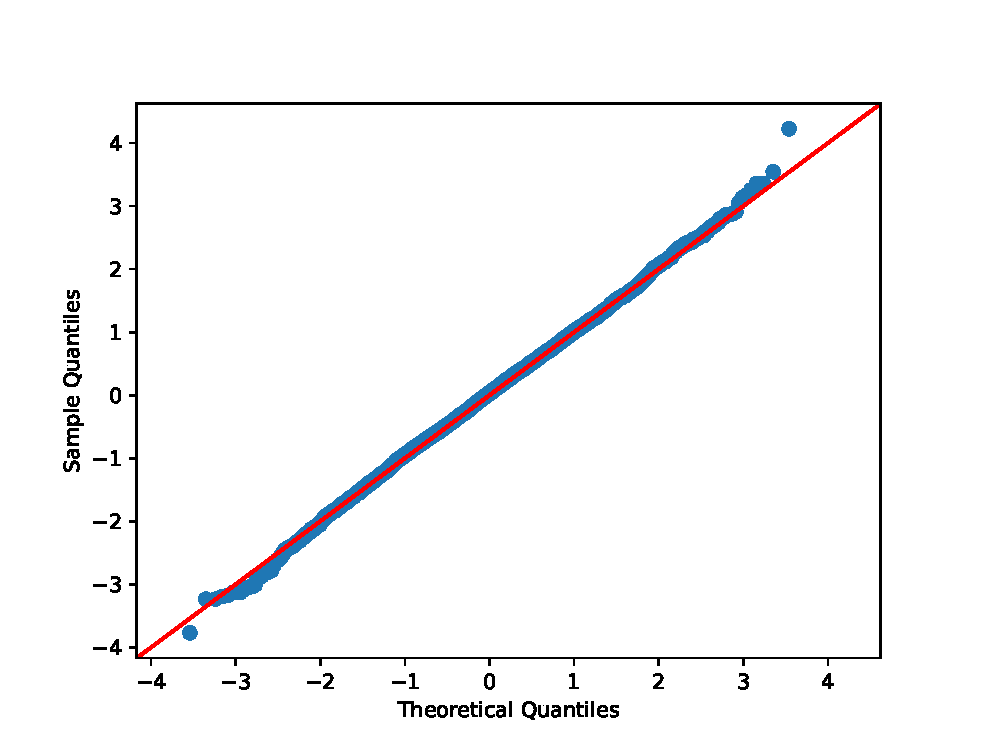
\includegraphics[ trim={10 0 0 30},clip, width=\linewidth]{qq.eps} 
\caption {QQ-plot of combined PRS, clearly distributed normally }\label{fig:qq}
}\end{figure}

It is possible to select a couple of SNPs including their direction (risk/non-risk allele) and calculate a score. If the score is extreme it indicates predictive power (in positive or negative way), while scores near 0 indicate low predictive power.\\


\begin{figure} [!h] \centering{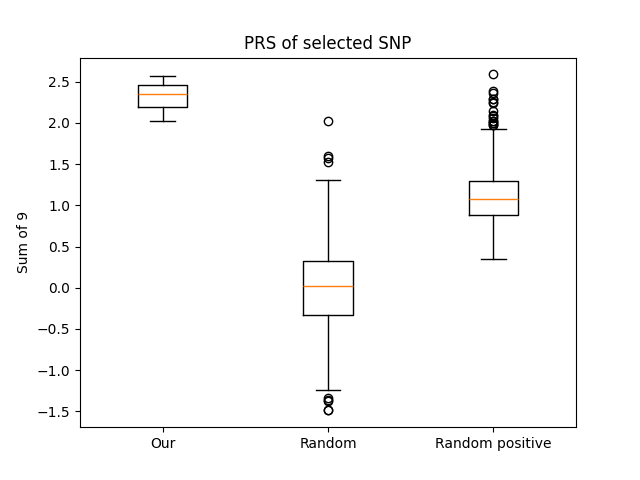
\includegraphics[ trim={0 0 0 20},clip, width=\linewidth]{PRS_selected} 
\caption {Boxplot of PRS of different selections with same size, our selections stem from the pyramid scheme, they deviate significantly from a random selection. }\label{fig:boxplot}
}\end{figure}

\begin{figure} [!h] \centering{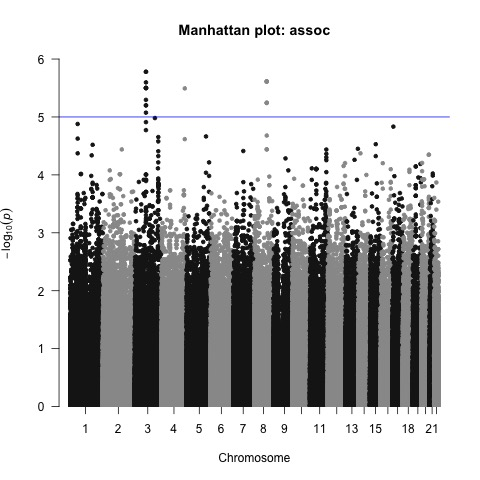
\includegraphics[ trim={0 10 0 20},clip, width=\linewidth]{Manhattan_PRS} 
\caption {Manhattan plot of our toy data }\label{fig:manhattan}
}\end{figure}

For the purpose of analyzing the combined predictive power of SNPs the PRS is not a particularly effective metric. It only states the individual predictive power, which may be obfuscated by balancing out effects. Generally, a high PRS indicates that  some SNPs with high predictive power have been found, but it is not required that they are balanced (unrelated) and therefore low scores should a priori not indicate a failure of the method. \\


\subsection{Products}
The output from Espresso is given as one line per product. The amount of products can be used as an indication of how many subgroups there are needed to find a minimal cover.

Generally, we assume less products in the result to be preferable as this can be seen as simpler relationship, which we deem to be more probable to fit the real cause. \\

It should be analyzed what impact each of the products have if there are multiple products, eventually it might prove necessary to discard some products which are specifying only to one small subset, while other products are true for many subjects. This is to avoid overfitting by stratifying to fit the given data perfectly but not the out-of-sample data.

If multiple products with considerable sizes (for in- and out-of- sample data) deviate in many SNPs, it can be speculated that two different groups being affected by different subtypes of diseases were classed into one single phenotype. This is especially interesting when multiple causes or outcomes are suspected. 
\subsection{Literals}
The amount of literals like for products indicates how complex the found solution is, again we prefer the simplest solution as we deem if to fit the real causes with a higher chance.
\subsection{Time \& Complexity}
Since the complexity of our approach is high, it is inevitable to consider it as part of the evaluation. An easy measure of the complexity is the time it took us to run the program. Change of dataset, parameters or computational  capabilities all have an influence on the time.
\section{ Tried methods}
Since no literature exists, nor do we have an already working method, we have to build it ourselves. Since most of the algorithms used do not change between the methods, we try to build up an infrastructure relying on the already built methods and modifying them to support additional methods or use the prebuilt block for building new blocks. 
\subsection{Primitive approaches}
Some methods seem to be trivial, but they will never work with our dataset. Nevertheless is it a good idea to consider those approaches as they might help us understand the more complex methods.
\subsubsection{Entire}
Taking the entire dataset and let Espresso try to find a minimal cover is impossible as the time requirements grow exponentially, as we know the problem for finding the minimum cover is not even in P. 

For small datasets, it might be possible and useful, though wrong genotyping or incorrect phenotypes will remain hidden. Another approach could be to filter more strictly in an attempt to decrease the size of the dataset.  

If previous knowledge exists suggesting that the result is made up by a single product, we could apply a filter and excluded all positions where the subjects having the phenotype differ as this makes it unsatisfiable if it were in the cover. 
\subsubsection{Omitting parts of the dataset}
\label{sec:omit}
Taking partial parts of the dataset and never discovering other parts is possible though it is highly doubtful how a satisfying solution can even be found consistently. For discovering the dataset and experimenting with different encodings, we did run some experiments. In the context of this experiment when we refer to $n$ we mean the amount of SNPs. 

\begin{enumerate} 
\setcounter{enumi}{3}
\item High $n$ yield a smaller product, we explain deviations from this rule by the diverging paths taken in Espresso or in case of different dataset by the difference of possibilities. 
\item Same as for products, just more pronounced as in practice this are higher numbers and therefore more possible outcomes (events) exist. 
\item This analysis is fast and easy to execute for small n, it scales exponentially with n. 
\end{enumerate}


The following table gives an overview of the acquired results with all 109 subjects considered. Each SNP is decoded as two digits, hence the input size is double the amount of selected SNPs. The results are averaged, estimated and depend on the selection of the SNPs. Here the selection was done randomly.  We might use those results as baseline assumptions in further experiments:

\begin{center}
\begin{tabular}{ c| c| c| c}
 \textbf{Input size (2n)} & \textbf{Products} & \textbf{Literals} & \textbf{Time} \\ \hline
 $<$120& -&-&$<$ 1s\\
 200 & 50 & 3-6&5s\\  
 400 & 40 & 2-4  & 10s \\
 1000& 30&2-3&40s\\
 2000&25&2&8min
\end{tabular}
\end{center}
\begin{figure}[!ht]
\centering{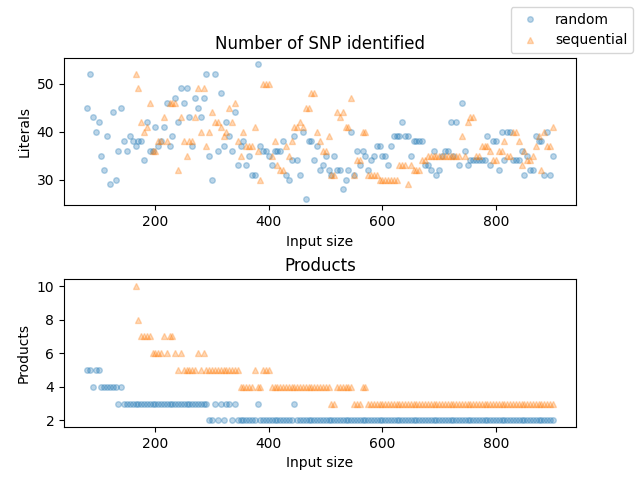
\includegraphics[width=\linewidth]{randseq} \caption {Comparison between random and sequential selection methods }\label{fig:randseq}
}
\end{figure}
\begin{figure}[!h] \centering{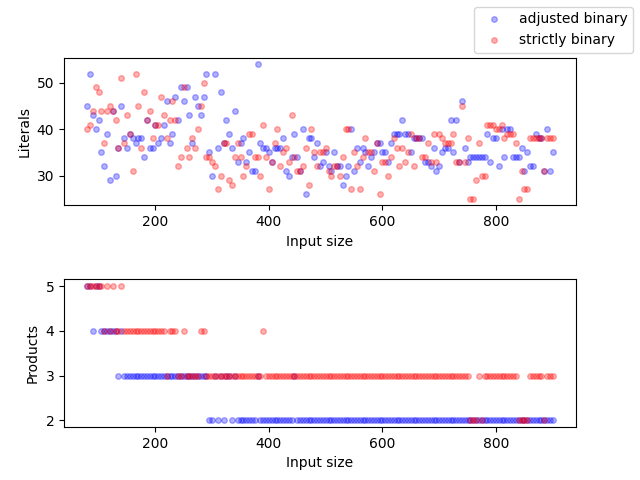
\includegraphics[width=\linewidth, trim={0 0 0 4},clip]{binarycomp} 
\caption {Comparison between different binary encoding methods }\label{fig:binary}
}\end{figure}
For a random selection with less than 60 SNPs, we can generally not find a cover as the truth table is over-specified. \\

A random selection of SNPs generally decreases the identified products required for a minimal cover compared to a sequential selection. This trend also affects the literals but is less pronounced. Additionally, it was discovered that in sequential analysis even for a relative high $n$ it might not be possible to find a cover due to over-specification. This is due to missing data not being distributed equally among the data, causing regions with high missingness ratio. This constitutes less of a concern for random selection, as in QC we filtered to have at an average of at most 2\% missingness. 

The random method will be used exclusively in all future analysis as we deem it to yield the better results for our purposes. 


Different encoding methods (see \ref{sec:encode}) also influence the result. The adjusted method is selected for the rest of this document. 




\subsubsection{Iterative approaches}
\begin{figure} [!h] \centering{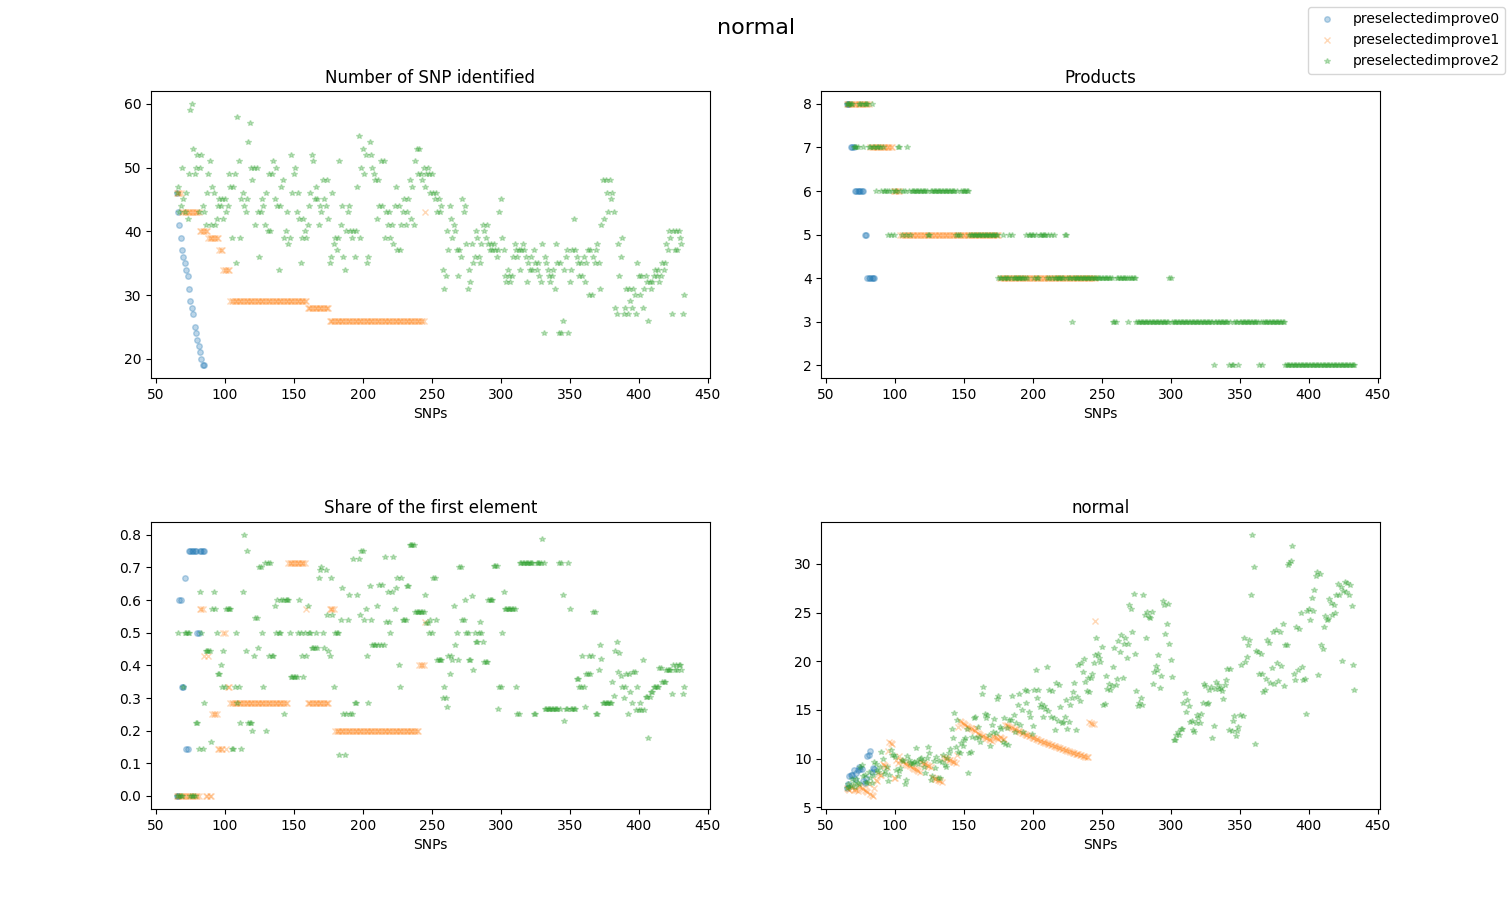
\includegraphics[ trim={70 320 0 0},clip, width=\linewidth]{play_snp} 
\caption {Iterative approaches with SNP indicating the number of selected SNPs, the limit was set on literals. 0: strictly decreasing, 1: monotonically decreasing, 2: no equivalences (increasing or decreasing)}\label{fig:play}
}
\end{figure}
We can try to start with some small selection and iteratively build up until the entire data set is included. We start with the smallest possible set such that the truth table is not over-specified and add one SNP, we evaluate this table, find a minimal cover and from the number of literals in the minimal cover, we decide whether this SNP stays in the selection depending on some criteria. Then we do same for every SNP until all SNP were included at one point. 

The time required to go through the entire dataset is immense, we are not able to tell Espresso what covers we already found and therefore we do not gain anything from the iterations before.  From some point onwards there are likely no gains as the best solution is a local minima of only a few SNPs.This approach does not consider all possible relationships between different SNPs. In fact, it only remarks the ones with a strong PRS anyways or a  tendency towards the starting set, making this approach not equilibrated. Furthermore, we are not guaranteed by Espresso to have an optimal minimal cover.

\subsection{Pyramid scheme}
In the pyramid scheme, the algorithm runs sequentially through the entire dataset by separating all SNPs into groups of size $k$, finding a minimal cover for every group. All the SNPs making part of a found minimal cover are then subsequently taken to the next level. This is repeated until in one level  all the identified SNPs from the previous level are less than k SNPs, from where a minimal cover for the entire universe of less than k SNPs can be found. \\

The selection of the group can be done in many ways, we decided to analyze the random selection approach as well as sequential, which should correspond to the sequences in the DNA as already explained in Chapter \ref{sec:omit}. We found random selection to be clearly preferable as we can see in Figure \ref{fig:randseq} and also because of the missingness problem with sequential selection.
We can either reshuffle the found SNPs or respect the order to preserve the relations from the previous level. We found that in-level shuffling yields slightly better results compared to preserving the relations. With this method, there is a higher probability for any two SNP to be in the same group which is not in the last level, but it also means that potential relations on a previous level are disregarded. 
The group size is fixed, but to prevent a small leftover, the leftover SNPs are added to the last full group, which means the max size of this group is at most doubles minus 1. If the groups from the previous level are respected, every group was filled with SNPs block-wise from the previous levels, meaning that all groups have at least group size k but most have slightly more SNPs and the last group might have 2k plus the size of the last minimal cover of the previous level minus one. \\

The selection of our SNPs compared to a random selection is indicating that they do not belong to the same distribution. For example, 9 SNPs together gave 2.03 as PRS value, while for a random selection distribution we have normal distribution with $\mu =0, \sigma=0.23$ giving p=0.000024, a random positive selection has distribution of $\mu =1.1, \sigma=0.096$, therefore giving p=0.0033, see Figure \ref{fig:boxplot}.

  
\subsection{Grouping scheme}
\begin{figure} [!h] \centering{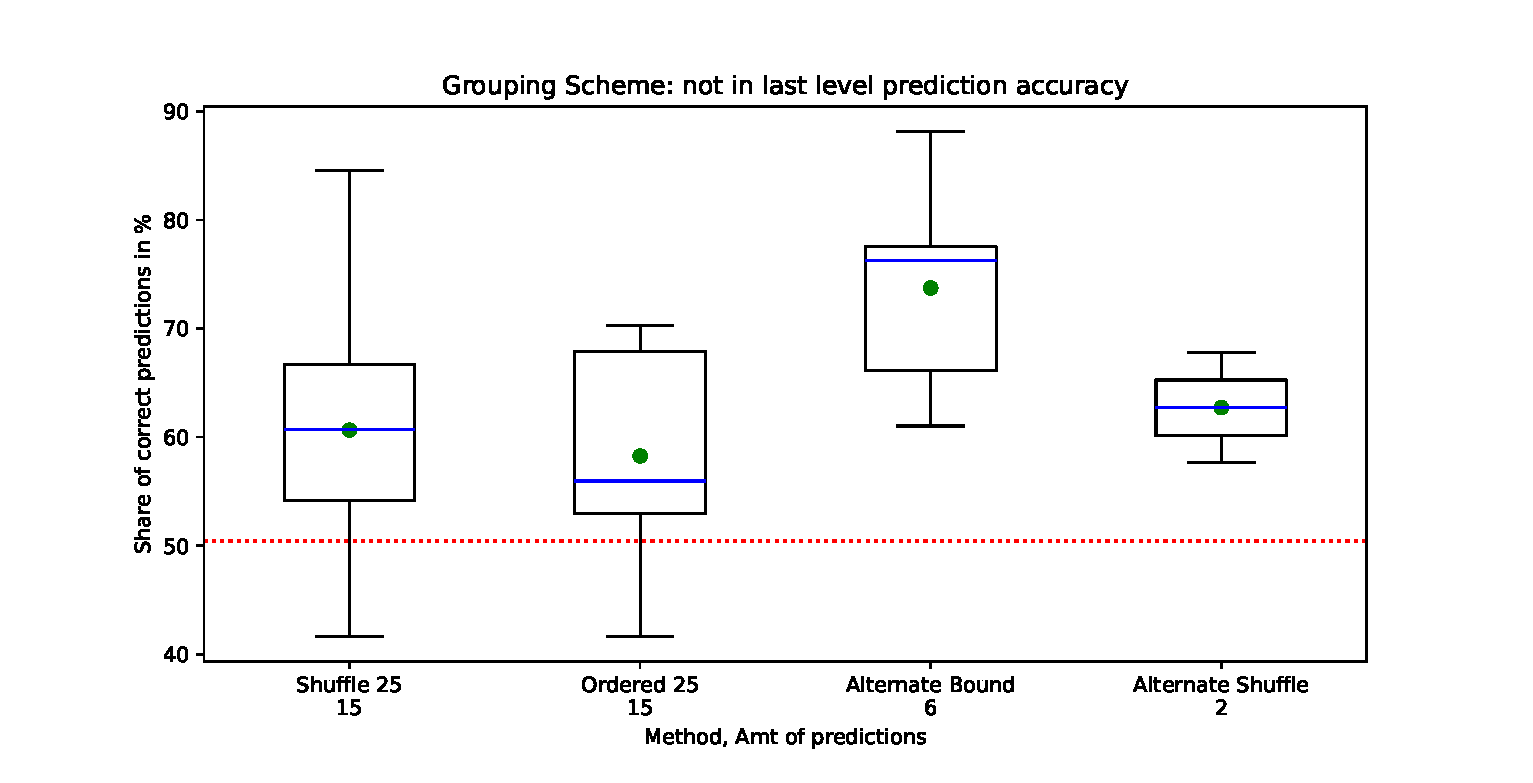
\includegraphics[ trim={0 0 0 0},clip, width=\linewidth]{selbox.eps} 
\caption {Prediction accuracies of the grouping scheme for the out of sample which means not in last level. Every category originally had 15 sample, because of over-specification some are eliminated, the updated count is displayed below the category name.   }\label{fig:selbox}
}
\end{figure}
The grouping scheme method divides the individuals into different equal-sized groups. For each level one group is chosen and the dataset of only those individuals is considered, the rest is performed similar to the Pyramid scheme. 

On each level, only a part of the individuals is considered, this means, that the minimal cover is optimized only for those people. On the next level, different individuals get selected, we can assume their phenotype is determined by the same underlying structure, therefore the previous minimal covers should suffice to find a minimal cover. If this is not the case, we have an over-specified truth table, this might be due to there not being an underlying structure or the missing detection of it or due to errors in genotyping. 
As for the pyramid scheme, we tested two methods for passing SNPs down a level and found the same preference for random shuffling in every level.  We use the same ruleset for overflow or leftover SNPs. \\

We found group sizes of 25\% of the in-sample data to be fitting for the approach with our initial dataset. With alternating groups, such as when splitting the individuals into two groups (group sizes of 50\%), the method yields lower prediction accuracies than the Pyramid scheme or 25\% group sizes. We suspect it  was optimizing for the in-sample data. Additionally, alternating often fails due to over-specification especially if the order from the previous level is not respected (shuffle SNPs after each level).\\

Later, the code was changed to refer to the selection of individuals of the previous level if the final analysis is over-specified. This should resolve most cases where over-specification was still posing a problem. We maintain the stance the randomization between the levels is preferable as this allows for more diverse range of combinations.\\

With the blood lipid dataset, we found that the result consists of about 9 products out of over 100 distinct SNPs ($k=500$), still with out-of-sample accuracy barely above 50\%. We had to increase $k$ (group size) as else we would have problems with over-specification. We increased it to 300/500, from which we concluded, that it should be increased even further, with $k=300$ it took 8 levels, but with $k=500$ only 5. Another complication is the time, for example with $k=500$ it took us more than one week to run a single experiment. Decreasing the percentage of group sizes, here 25\% could be appropriate for improving the results.

\section{Creating data with given structure}
In this chapter we try to evaluate what is possible to achieve with our method and what has to be expected simply by random occurrences. We simulate or change data such that we have a more direct correspondence, which we can try to predict. This gives us an understanding of the capabilities of our methods.
\subsection{Phenotype shuffling}
We shuffle the phenotypes of all the individuals, this is achieved through random selection of k persons which have phenotype 2 respectively 1. This preserves $p$ of having the phenotype. 
This altered dataset can be run to test different methods. When this is done we expect the resulting minimal cover to be random. 
Our method where structure exists, should need less literals or products as there is an underlying structure dictating the outcome, while this is obviously not true for shuffled phenotypes. We can also check the frequencies of the selected SNPs with shuffled phenotypes to see whether there exists an overlap with the SNPs of our normal method. If this were to be the case repeatedly, this  would hint at a problem in our method potentially stemming from the fact that identifying individuals with certain SNPs is easy, which we generally do not want as this would be overfitting.\\
It was found that not all schemes support phenotype shuffling. For example the grouping scheme relies on the fact that there is some underlying structure determining the phenotype from the  genotypes. It was observed that over-specification might occur that since due to the phenotypes being random attributed. This causes the SNP from a previous level to be nearly entirely insignificant. \\


\subsection{Introducing artificial diffusion based on specific criteria}

We would like to test how multiple underlying products affect the data. Unfortunately, the available test data only requires one product. If we change the phenotype of all persons based on some specific genotype variation, we hope to see this exact configuration in the results. Furthermore, we expect two products of which one is composed of our chosen diffusion criteria and to be closely related to a valid minimal cover for the original data. Further alterations or even combining of phenotypes might proof to be useful not only for evaluating the results but also for analyzing phenotypes with considerable pleiotropy or suspected subtypes.

We could not replicate the expectations in any of the 5 run experiments. We run the experiment with the grouping scheme with group sizes of 25. We diffused the phenotype by oring the phenotype with the pairwise selection of a specific SNP. This replaced phenotype, we expect to have the same minimal cover plus an additional product containing the specific SNP.  
\subsection{Simulated data with given phenotype-genotype relations}

We create a simulated dataset. For simplicity, we attribute only A (risk) and G (norisk) for all SNP not used for the phenotype generation, while C (risk) and T (norisk) serve for SNP determining the phenotype. This does not have an influence on the results as we encode them independent of the actual letter. Each SNP (with some caveats for  the determining SNPs), gets attributed a random MAF uniformly distributed between 5\% and 50\%. \\

We mostly tested with the same size as our initial dataset. If less anded 3 SNPs determine the SNP, our methods find this exact cover. Adding more anded SNPs, gives as result only a subset of all determining SNPs with 3 identified SNPs. Apparently they suffice for a minimal cover, repeated tests could unveil more SNPs, identification with the histogram should be possible. 
Oring the determining SNPs for the phenotype failed to be detected even with only 1 SNP per product. This is due to a limitation in Espresso, which needs to be investigated further. 

\section{Evaluation of the methods}%Discussion
\begin{figure} [!ht] \centering{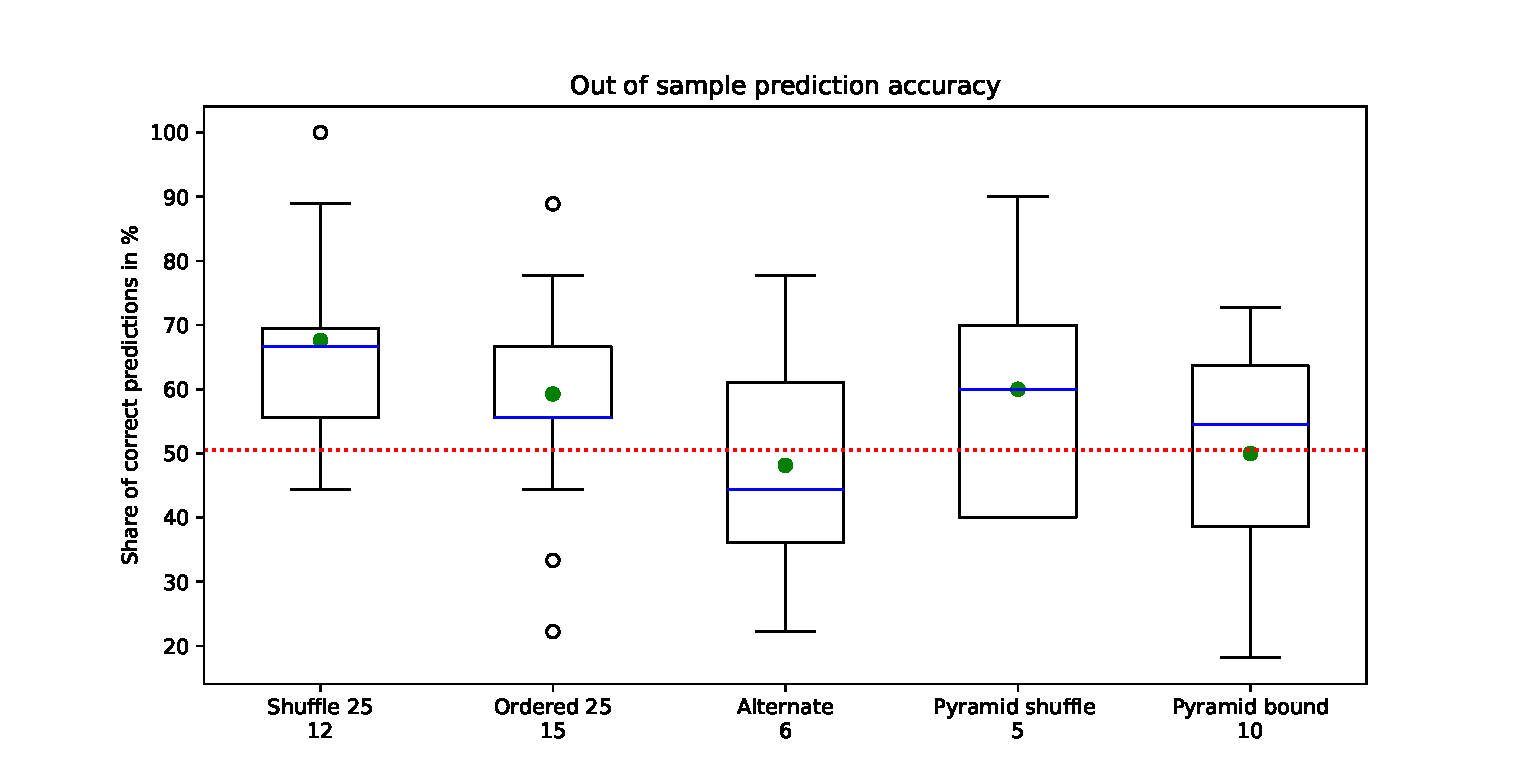
\includegraphics[ trim={0 0 0 20},clip, width=\linewidth]{accuracyplot.eps} 
\caption {Prediction accuracies of  predicted outcomes in data out of sample data, never included in the data before. The red lines indicates the expected guessing accuracy for this data with a random approach. The data is theoretically continuous, here we observe the out-of-sample size to be too small (about 10) , explaining the occurrences of overlapping quartiles and medians.}\label{fig:accuracy}
}
\end{figure}
\begin{figure} [!ht] \centering{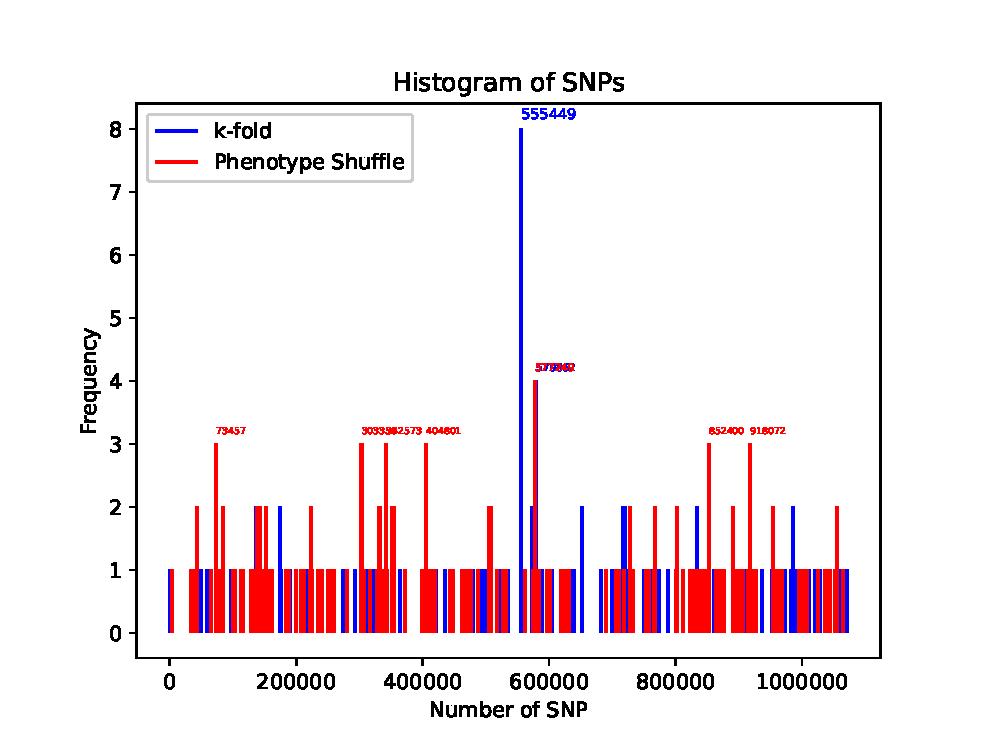
\includegraphics[ trim={10 0 0 20},clip, width=\linewidth]{histall.eps} 
\caption {Histogram of multiple k-folds using one out of pyramid scheme, grouping scheme or phenotype shuffling schemes. The grouping scheme is superimposed on top of the k-fold. No overlap is detected, clear trends with the pyramid scheme are visible, while for shuffled phenotypes no order is apparent.   }\label{fig:frq}
}
\end{figure}


From the out-of-sample prediction accuracy, we determine that some approaches perform better than random, though we would hope for higher accuracy. It is apparent, that improvements are required or rather that a single cover does not suffice to make any kind of prediction.\\

We consistently see some of the SNPs reappearing in different covers, which might signal the importance of that specific SNP. For shuffled phenotypes, this phenomena was not observed, hence there is no selection which is generally good for identifying persons. 

This result is expected and supports the claim of significance of the found SNPs.\\

The histogram seems less crowded than the Manhattan plot of the PRS of Figure \ref{fig:manhattan}. Also most of the SNP have a high PRS value indicating correlation with the phenotype. Repeated results are a sign of confidence, but it also needs to be mentioned, that we are far away from having equal results in all iterations. This also indicates that potentially multiple global optima exist or it has not even been found yet.  Except for  the pyramid scheme there does not exist clear "favorite" SNPs but rather a small collection of SNPs appearing more than once.

Another question is whether the global optima or any found cover for this purposes actually has biological credibility in explaining the surveyed phenotype. \\

The final method, we claim works the best using Espresso for our test-data has following properties: QC completed, binary translation adjusted with $2_{10}=11_2$, randomization for the selection of 200 SNPs for the start as well as between the levels, using the grouping scheme with 25\% of the total population per group, allow at most 30 unknowns before cutting individuals, which in fact does not happen, not checking for over-specification as it does not happen either. 
\section{Future potential}%Conclusion
This research is severely limited by the availability of data and the capabilities of Espresso. Encoding the problem with ternary encoding might improve accuracy. Although, we did not achieve to find a way in which this can be, we believe there exists some structures to support  multivalued inputs with Espresso. Additionally, we could increase the confidence for combinations including ors by using SMT solver instead of heuristic Espresso. If this is feasible, we would be able to identify more responsible SNP in more complex circumstance, as long as they solely and entirely determine the phenotype. Analysis of the products could detect different undetected subtypes of a disease and allow for separation of those types.  \\


The method succeeds at finding risk loci, but as of now, it fails in correctly predicting the phenotype. Better datasets and tools might increase the reliability but PRS remains strong in predicting on an individual level. Our approach would be more fit for identifying the cause of disease and therefore be a tool for use in research. 

If the method is not able to find minimum covers, this might be due to a violation of the initial assumptions or in particular because the phenotype cannot be fully explained through genetics. We do not see this as a bug but rather a feature.\\

Machine learning algorithms could be also be involved. Hybrid versions, which evaluate PRS as well as relations between SNPs, should be investigated. The histogram of Figure \ref{fig:frq} could also be interpreted as a refined version of a Manhattan plot. The heights of the points in the Manhattan plot could be added to create a new combined evaluation. 


\newpage
\begin{thebibliography}{99}
\bibitem{tutorial}
\emph{Marees AT et al. } A tutorial on conducting genome-wide association studies: Quality control and statistical analysis. \url{https://pmc.ncbi.nlm.nih.gov/articles/PMC6001694/}
\bibitem{lipid_data}
\emph{Hajiaghabozorgi, M. } GWAS dataset with simulated binary phenotypes for 1000 Genome Project. March 1, 2023. \url{https://doi.org/10.5281/zenodo.7683384}
\bibitem{1k}
\emph{The 1000 Genomes Project Consortium.} A global reference for human genetic variation. Nature 526, p. 68–74. 2015.\url{ https://doi.org/10.1038/nature15393}
\bibitem{prs}
\emph{Teri Manolio} National Human Genome Research Institute (NIH). August 19 2025. \url{https://www.genome.gov/genetics-glossary/Polygenic-Risk-Score-PRS}
\bibitem{10ygwas}
\emph{Peter M. Visscher et al. } 10 Years of GWAS Discovery: Biology, Function, and Translation, The American Journal of Human Genetics . July 6 2017, p 5-22. 
\end{thebibliography}
\end{document}